\chapter{Аналитическая часть}

В этом разделе будут рассмотрены, виды симметричного шифрования, алгоритмы перестановки и подстановки, криптографический алгоритм DES.

\section{Виды симметричного шифрования}

Симметричное шифрование делится на два основных вида: поточное и блочное. В поточном шифровании данные обрабатываются побитово или посимвольно, в то время как в блочном шифровании данные разбиваются на блоки фиксированного размера.

\begin{itemize}[label=---]
    \item \textbf{Поточное шифрование} --- шифрование происходит в реальном времени, каждый бит открытого текста шифруется независимо;
    \item  \textbf{Блочное шифрование} --- данные разбиваются на блоки фиксированной длины, и каждый блок шифруется отдельно.
\end{itemize}


\section{Алгоритм DES}

Шифровальная алгоритм DES (англ. \textit{Data Encryption Standart} --- DES) --- симметричный шифровальный алгоритм, разработанный в 1977 году компанией IBM. Он использует блочное шифрование, длина блока фиксирована и равна 64 битам. 
Однако каждые 8 бит в ключе игнорируются, что приводит к правильной длине ключа 56 бит в DES. 
Однако в любом случае один блок на 64 бита является вечной организацией DES.
Он состоит из 3 следующих шагов, рисунок~\ref{fig:des}: 
\begin{itemize}
	\item начальная перестановка (англ. \textit{Initial Permutation} --- IP), во время которой биты переставляются в порядке, определённом в специальной таблице;
	\item 16 раундов шифрования;
	\item завершающей перестановки (англ. \textit{Final Permutation} -- FP), соовершающей преобразования, обратные сделанным на первом шаге.
\end{itemize}

Раунд шифрования состоит из 5 следующих этапов
\begin{enumerate}[label=\arabic*)]
	\item расширение (англ. \textit{expansion} --- E);
	\item получение ключа раунда (англ. \textit{Round Key} -- RK);
	\item скремблирование (англ. \textit{substitution} --- S);
	\item перестановка (англ. \textit{permutation} --- P)
	\item смешивание ключа (англ. \textit{key mixing} --- KM).
\end{enumerate}

На рисунке~\ref{fig:des} представлена обобщенная схема шифрования алгоритма DES.

\begin{figure}[ht!]
	\centering
	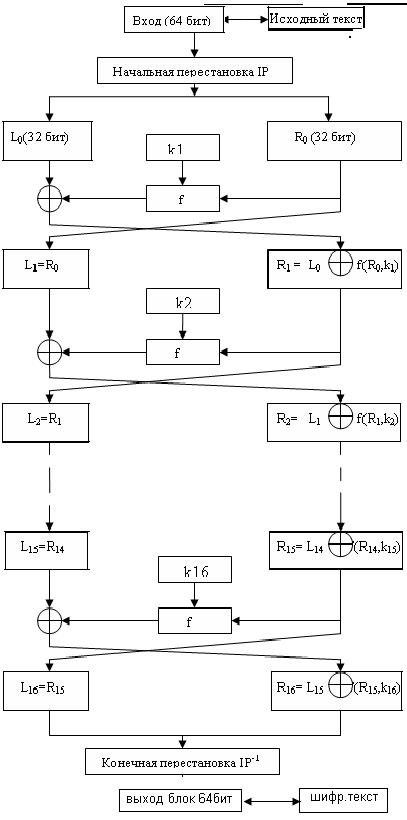
\includegraphics[width=0.4\linewidth]{images/des_scheme.png}
	\caption{Обобщенная схема шифрования в алгоритме DES}
	\label{fig:des}
\end{figure}

Расширение, во время которого каждая из половин блока шифрования по 32 бит дополняется путём перестановки и дублировоания бит до длины в 48 бит.

Получение ключа раунда необходимо для применения в раунде шифрования 48-битного ключа раунда, полученного из основного ключа DES. Основной ключ имеет длину 64 бита, однако значащих бит из 64 всего 56, остальные добавлены для избыточности и контроля передачи ключа. Из этих 56 бит получают 48 путём разбиения на равные части и применению битовой операции циклического сдвига и нахождению нового значения посредством специальной таблицы.

Скремблирование предназначено для получения из 48-битного потока 32-битного путём разбиения на 6 частей по 8 бит и обработки каждой части в S-блоках (англ. \textit{Substitution boxes}), которые заменяют блоки с длиной 6 бит на блоки 4 бит посредством использования специальной таблицы.

Перестановка представляет из себя перемешивания полученной последовательности из 32 бит при помощи таблицы перемешивания.

Смешивание ключа представляет из себя операцию XOR полученного 32-битного значения c ключом раунда.


\section{Режимы работы алгоритма DES}

Режим шифрования --- метод применения блочного шифра, позволяющий преобразовать последовательность блоков открытых данных в последовательность блоков зашифрованных данных.

Для DES рекомендованы следующие режими работы:
\begin{enumerate}[label=\arabic*)]
	\item режим электронной кодовой книги (англ. \textit{Electronic Code Bloc} --- ECB);
	\item режим сцепления блоков (англ. \textit{Cipher Block Chaining} -- CBC);
	\item режим параллельноого сцепления блоков (англ. \textit{Parallel Cipher Block Chaining} -- PCBC);
	\item режим обратной связи по шифротексту (англ. \textit{Cipher Feed Back} --- CFB);
	\item режим обратной связи по выходу (англ. \textit{Output Feed Back} --- OFB).
\end{enumerate}

В данной работе будет электронной кодовой книги (ECB).

\section{Алгоритмы перестановки и подстановки}

\textbf{Алгоритм перестановки} --- это метод шифрования, при котором биты входных данных перемешиваются в соответствии с фиксированной схемой. Порядок следования битов изменяется, но их значения остаются прежними. Пример: Initial Permutation в DES.

\textbf{Алгоритм подстановки} --- это метод шифрования, при котором биты или группы битов заменяются на другие значения согласно заранее определенной таблице замен. Пример: S-блоки в DES;

Алгоритм DES использует оба подхода.
